\documentclass{article}
\usepackage{math}
\usepackage{tikz}
\usetikzlibrary {arrows.meta}

\title{An Introduction to Category Theory}
\author{Andrew L Jones}\date{}

\begin{document}
\maketitle

% INTRODUCTION

\section*{Introduction}
One of the most abstract fields of mathematics: Category Theory arose from the practice of representing relations as diagrams on blackboards. Although its origins might be in the corporeal world of chalkboards and erasers, Category Theory is a field of mathematics that emphasizes the abstract study of mathematics as form over the applied use of mathematics as calculation. As Lawvere states, it "has long been felt in advanced algebra and topology, namely that the substance of mathematics resides not in Substance (as it is made to seem when $\in$ is the irreducible predicate, with the accompanying necessity of defining all concepts in terms of a rigid elementhood relation) but in Form" \cite{Lawvere01}. 

In more concrete terms, chasing the underlying fundamental Substances that can establish a foundation for mathematics might not be as fruitful as studying the forms that mathematics can take on. Category theory is a language that allows mathematicians to study mathematics as form.

% FIRST SECTION 

\section{Objects and Arrows}
Fundamental to this study of mathematical form is the concept of a Category.
\begin{definition}
A category consists of a Class of Objects $ob(c)$; a Class $mor(C)$ of Arrows; a source of Objects to map from $dom(C)$; a target of Objects to map to $cod(C)$. Categories must satisfy three conditions: \begin{enumerate}
    \item Arrows must be associative
    \item Arrows most compose with other Arrows
    \item All Objects must have a left and right identity that is part of the Arrows
  \end{enumerate}
\end{definition}
\subsection{Concrete Categories}
Arrows can be and usually are functions. Objects can be and usually are sets. Categories in which every Object is a set are called \textbf{small} categories. Categories in which every arrow is $id$ are called \textbf{discrete} categories.

\begin{theorem}
The Group $A(\mathbb{R}, +, *)$ is a \textbf{small} \textbf{discrete} category.
\end{theorem}
\begin{proof}
Let C be a category with $ob(C)=\{\mathbb{R}\}$ with $dom(C) = \mathbb{R}$ and $cod(C) = \mathbb{R}$. Let $a,b,c \in R$. For $+$ fix $e = 0$ and observe that $a + e = a$ and $e + a = a$. Observe that $(a+b) + c = a + (b+c)$. Likewise, for $*$ fix $e = 1$ and observe $a * 1 = a$ and $1 * a =a$. Observe that $(a*b)*c = a*(b*c)$. Hence, the Group $A(\mathbb{R},+,*)$ is a category.
\end{proof}

\subsection{Comparing Forests}
Given that \textbf{small} categories have sets as Objects, large sets such as the set of all sets $\Omega$ are small categories. Hence Category Theory can reason about large sets primarily using diagrams composed of Arrows, resulting in a field that is more about structure than content. To quote Herrlich and Strecker: "Category Theory involves the next level of abstraction-i.e., comparing forests." \cite{Herrlich01}. This abstraction goes so far that the actual value of the sets often matters less than the composition of arrows. As Milewski puts it: “Category theory is extreme in the sense that it actively discourages us from looking inside the objects. An object in category theory is an abstract nebulous entity.” \cite{Milewski01}. This level of abstraction only further reinforces the convention of representing categories as diagrams.

\begin{center}
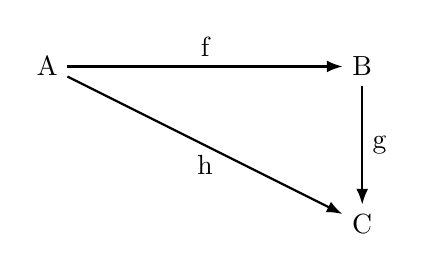
\begin{tikzpicture}
\path (-2,2) node (A) [black] {A};
\path (2,2) node (B) [black] {B};
\path (2,0) node (C) [black] {C};
\draw[thick, ->, -{Latex[length=2mm]}] (A) -- (B) node[midway,above] {f};
\draw[thick, ->, -{Latex[length=2mm]}] (B) -- (C) node[midway,right] {g};
\draw[thick, ->, -{Latex[length=2mm]}] (A) -- (C) node[midway,below] {h};
\end{tikzpicture}
\end{center}
In the above diagram we have $f: A \to B$, $g: B\to C$, $h = g \circ f$. As following $f$ to $g$ has the same result as $h$, we can claim this diagram commutes.

\begin{definition}
    A diagram \textbf{commutes} when all parallel arrows obtained by composing arrows in the diagram agree.
\end{definition}

% SECOND SECTION

\section{Functors}
Categories commute by composition of arrows hence Category Theory is the study of the form of those arrows. Therefore, the field contains many different types of Arrows. Functors are a type of Arrow that maps between Categories while preserving structure.
\begin{definition}
    Assume that $A$ and $B$ are categories. A Functor $F$ is a map between Categories such that:
    \begin{enumerate}
        \item Each Object from $A$ maps to an Object in $B$
        \item Each Arrow from $A$ maps to an Arrow in $B$ such that:
        \begin{enumerate}
            \item The identity arrows  $Id_A$ and $Id_B$ hold
            \item Preserves composition such that $F(f \circ g) = F(f)\circ F(g)$ where $f \in mor(A)$ and $g \in mor(B)$.
        \end{enumerate}
    \end{enumerate}
\end{definition}

\begin{theorem}
The function $F: x \mapsto |x|$ is a functor from $\mathbb{Z}$ to $\mathbb{Z_{\ge 0}}$
\end{theorem}
\begin{proof}
Fix $a,b \in \mathbb{R}$ and $f: x \mapsto ax$ and $g: x \mapsto bx$. Therefore $g \circ f = bax$. Hence, $F(g \circ f) = F(f) \circ F(g)$. Observe that $|bax| = |b|ax||$.
\end{proof}
\begin{center}
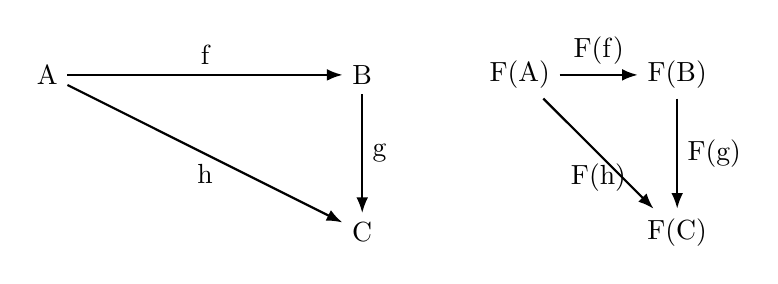
\begin{tikzpicture}
\usetikzlibrary {arrows.meta}
\path (-2,2) node (A) [black] {A};
\path (2,2) node (B) [black] {B};
\path (2,0) node (C) [black] {C};
\path (4,2) node (FA) [black] {F(A)};
\path (6,2) node (FB) [black] {F(B)};
\path (6,0) node (FC) [black] {F(C)};
\draw[thick, ->, -{Latex[length=2mm]}] (A) -- (B) node[midway,above] {f};
\draw[thick, ->, -{Latex[length=2mm]}] (B) -- (C) node[midway,right] {g};
\draw[thick, ->, -{Latex[length=2mm]}] (A) -- (C) node[midway,below] {h};
\draw[thick, ->, -{Latex[length=2mm]}] (FA) -- (FB) node[midway,above] {F(f)};
\draw[thick, ->, -{Latex[length=2mm]}] (FB) -- (FC) node[midway,right] {F(g)};
\draw[thick, ->, -{Latex[length=2mm]}] (FA) -- (FC) node[midway,below] {F(h)};
\end{tikzpicture}
\end{center}
Therefore the diagram commutes.

% BIBLIOGRAPHY

\bibliographystyle{plain}  % see:  https://www.overleaf.com/learn/latex/Bibtex_bibliography_styles
\bibliography{testbib}
\end{document}

